\documentclass{standalone}
\usepackage{tikz}
\usepackage{ctex,siunitx,ninecolors}
\setCJKmainfont{Noto Serif CJK SC}
\usepackage{tkz-euclide}
\usepackage{amsmath}
\usepackage{wasysym}
\usetikzlibrary{patterns, calc}
\usetikzlibrary {decorations.pathmorphing, decorations.pathreplacing, decorations.shapes,}
\begin{document}
\small
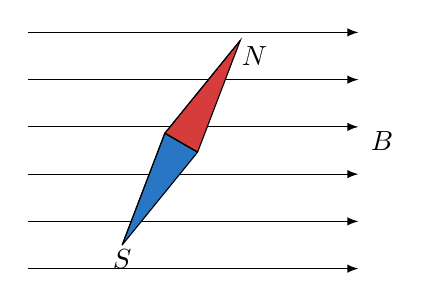
\begin{tikzpicture}[>=latex,scale=0.6]
  \useasboundingbox(-2,-0.6)rectangle(6,4.6);
  \foreach \x in {-.5,.5,...,4.5}
  {
     \draw [->](-2,\x)--(5,\x);
  }
  \draw [rotate=60, fill=red5](2.5,-.4)--(2.5,.4)--(5,0);
  \draw [rotate=60, fill=azure5](2.5,-.4)--(2.5,.4)--(0,0);
  \draw [rotate=60](0,0)--(2.5,-.4)--(5,0)--(2.5,.4)--(0,0);
  \draw [rotate=60](2.5,-.4)--(2.5,.4);
  \node at (0,-.3){$S$};
  \node at (2.8,4){$N$};
  \node at  (5.5,2.2){$B$};
\end{tikzpicture}
\end{document}